\section{Distribución normal}
\subsection{Definición}
Sea $f$ una función de distribución $x$ una variable aleatoria con media $\mu$ y varianza $\sigma^2$, entonces:
\begin{equation}
    P(x;\mu,\sigma) = \frac{1}{\sigma\sqrt{2\pi}} e^{-\frac{1}{2}\left(\frac{x-\mu}{\sigma}\right)^2} \qquad x\in \mathbb{R}
\end{equation}
\begin{figure}[H]
    \centering
    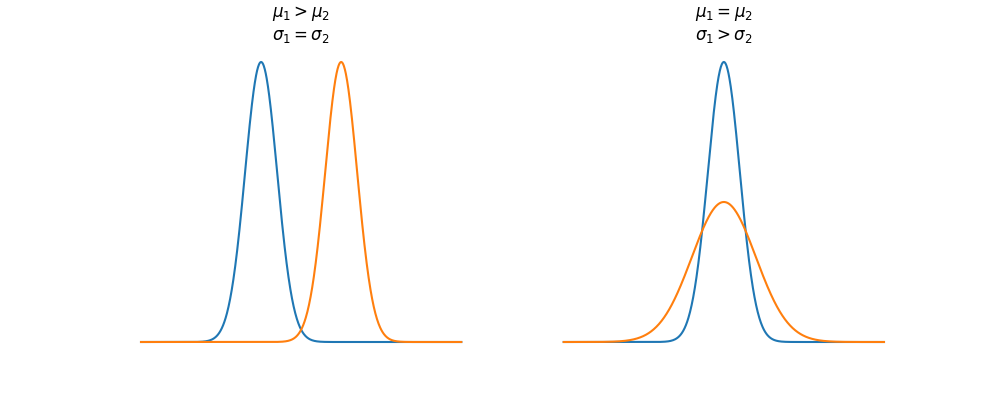
\includegraphics[scale=0.6]{Graphics/Normal_distribution.png}
    \caption{Ejemplos de distribuciones normales}
\end{figure}
Por convención se definio la variable $z$ como
\begin{equation*}
    z= \frac{x-\mu}{\sigma}
\end{equation*}
donde $z=0$ es el punto máximo de la gaussiana.
\subsection{Tabla normal estandar}
\begin{ejemplo}
    Hallar el área bajo la curva NORMAL en cada uno de los siguientes casos.
    \begin{enumerate}
        \item Entre z=0 y z=1.2.
              \begin{align*}
                  P(0\leq z\leq 1.2) = 0.3849
              \end{align*}
              \begin{figure}[H]
                  \centering
                  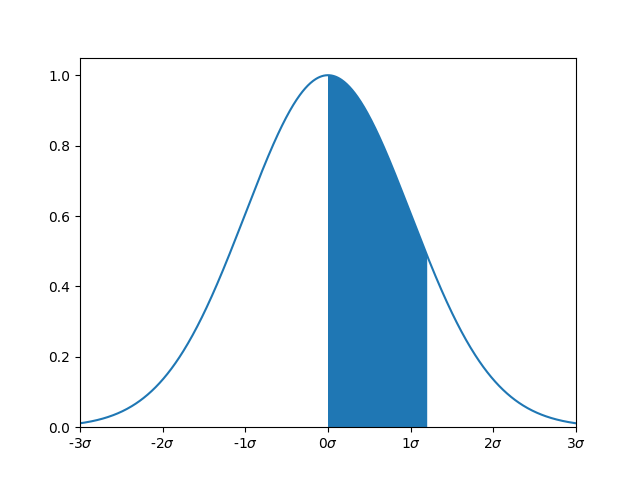
\includegraphics[scale=0.4]{Graphics/ejemplo_1.png}
              \end{figure}
        \item Entre z=-0.68 y z=0.
              \begin{align*}
                  P(-0.68\leq z\leq 0) & = P(0\leq z \leq 0.68) \\
                                       & = 0.2518
              \end{align*}
              \begin{figure}[H]
                  \centering
                  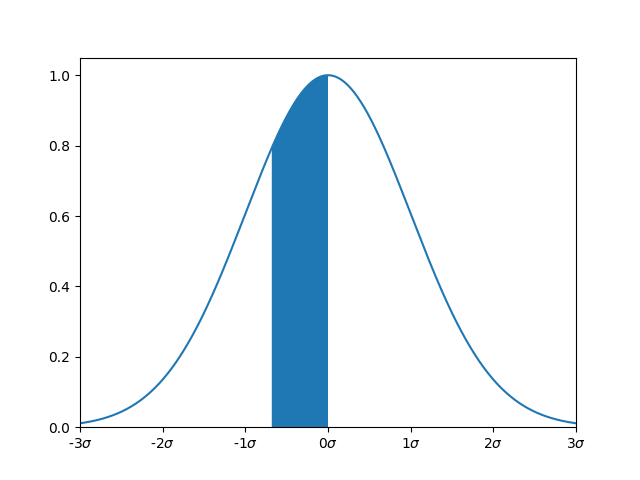
\includegraphics[scale=0.4]{Graphics/ejemplo_2.png}
              \end{figure}
        \item Entre z=-0.46 y z=2.21.
              \begin{align*}
                  P(-0.46\leq z\leq 2.21) & = P(0\leq z \leq 0.46)+P(0\leq z \leq 2.21) \\
                                          & = 0.1772+0.4864                             \\
                                          & =0.6636
              \end{align*}
              \begin{figure}[H]
                  \centering
                  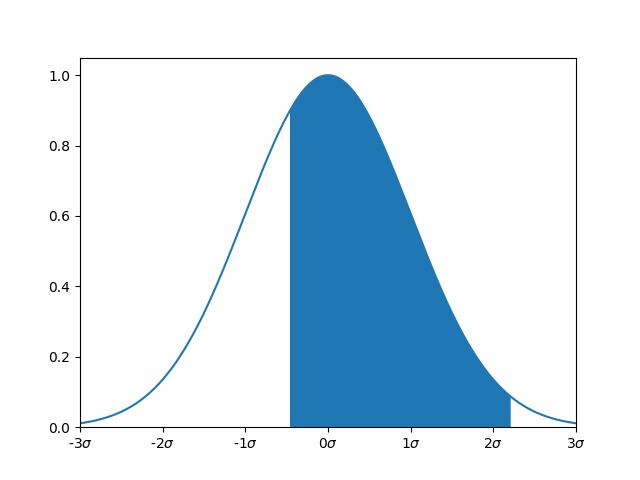
\includegraphics[scale=0.4]{Graphics/ejemplo_3.png}
              \end{figure}
        \item Entre z=0.81 y z=1.94
              \begin{align*}
                  P(0.81\leq z\leq 1.94) & = P(0\leq z \leq 1.94)-P(0\leq z \leq 0.81) \\
                                         & = 0.4738-0.2910                             \\
                                         & =0.1828
              \end{align*}
              \begin{figure}[H]
                  \centering
                  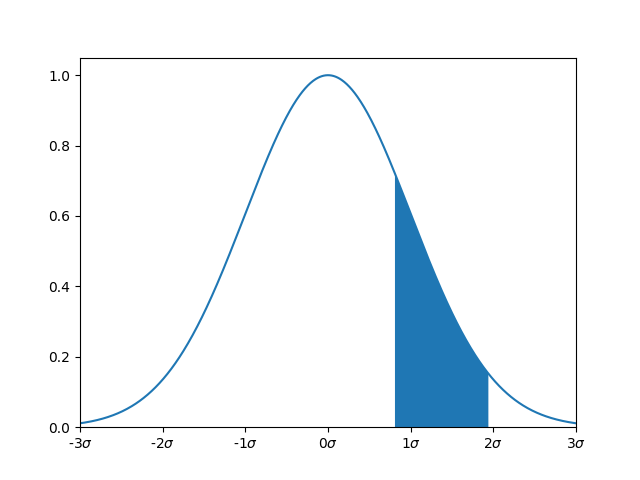
\includegraphics[scale=0.4]{Graphics/ejemplo_4.png}
              \end{figure}
        \item A la izquierda de z=-0.6
              \begin{align*}
                  P(z\leq -0.6) & = P(z \geq 0.6)            \\
                                & =0.5 - P(0\leq z \leq 0.6) \\
                                & = 0.5 - 0.2258             \\
                                & =0.2742
              \end{align*}
              \begin{figure}[H]
                  \centering
                  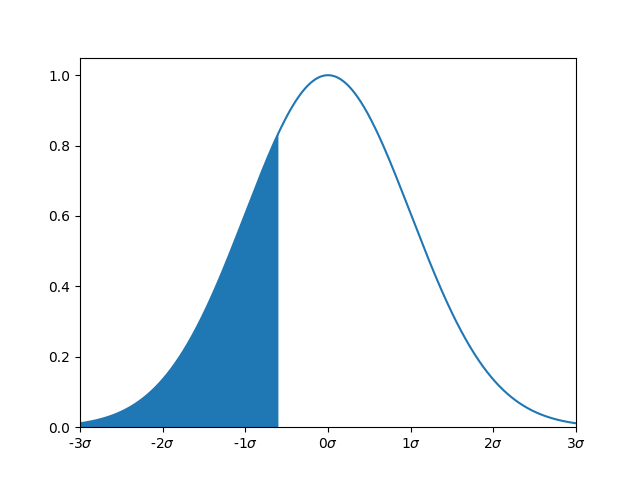
\includegraphics[scale=0.4]{Graphics/ejemplo_5.png}
              \end{figure}
        \item A la derecha de z=-0.128
              \begin{align*}
                  P(z\geq -0.6) & = 0.5+ P(0\leq z \leq 1.28) \\
                                & =0.5 + 0.3997               \\
                                & = 0.8997
              \end{align*}
              \begin{figure}[H]
                  \centering
                  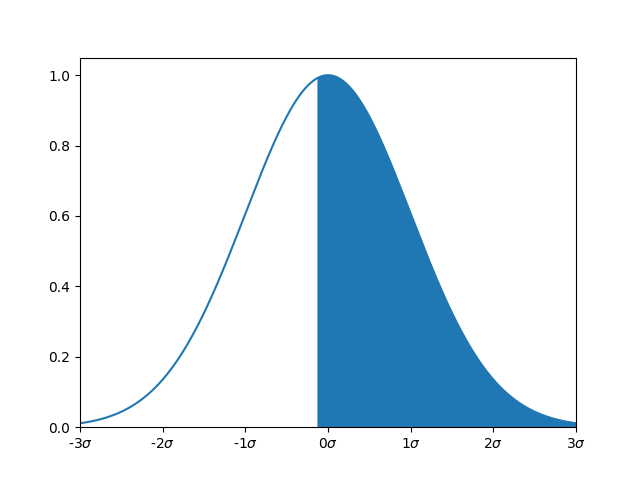
\includegraphics[scale=0.4]{Graphics/ejemplo_6.png}
              \end{figure}
    \end{enumerate}
\end{ejemplo}